\section{Model2DRigid\-Car  Class Reference}
\label{class_Model2DRigidCar}\index{Model2DRigidCar@{Model2DRigid\-Car}}
A rigid car-like robot in a 2D world. 


{\tt \#include $<$model2d.h$>$}

Inheritance diagram for Model2DRigid\-Car::\begin{figure}[H]
\begin{center}
\leavevmode
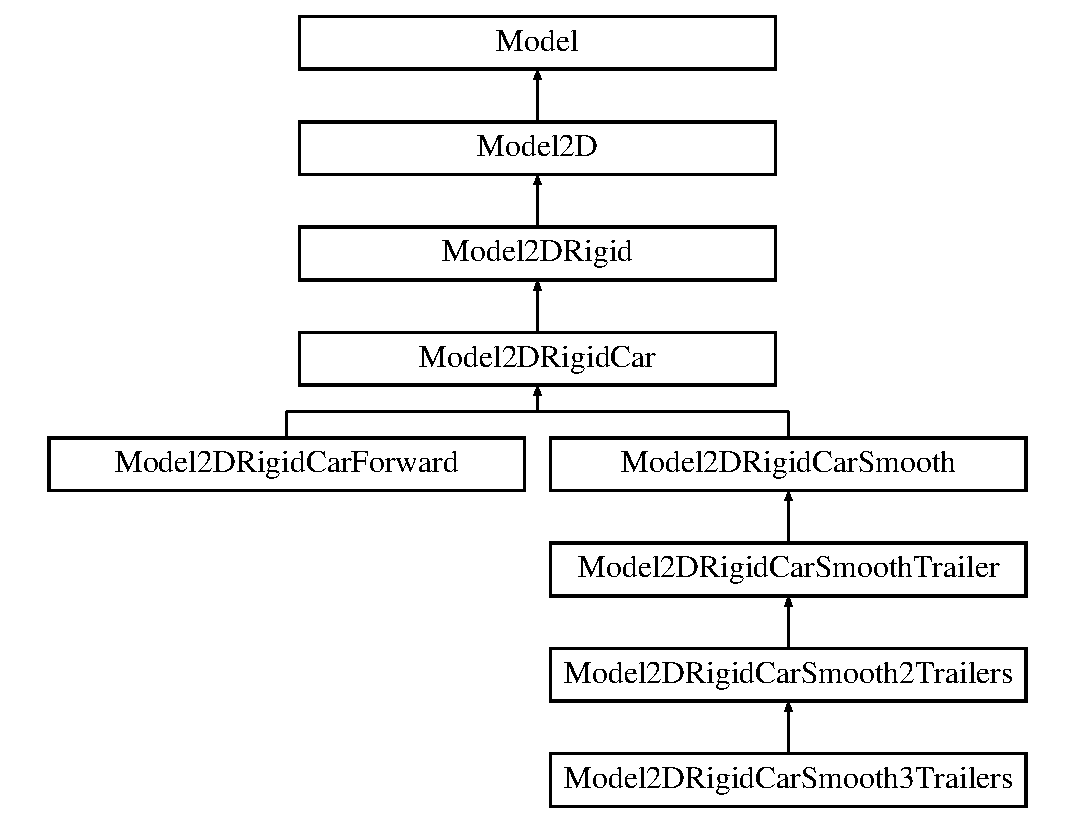
\includegraphics[height=8cm]{class_Model2DRigidCar}
\end{center}
\end{figure}
\subsection*{Public Methods}
\begin{CompactItemize}
\item 
{\bf Model2DRigid\-Car} (string path)
\item 
virtual {\bf $\sim$Model2DRigid\-Car} ()
\item 
virtual {\bf MSLVector} {\bf State\-Transition\-Equation} (const {\bf MSLVector} \&x, const {\bf MSLVector} \&u)
\begin{CompactList}\small\item\em The state transition equation, or equations of motion, xdot=f(x,u).\item\end{CompactList}\end{CompactItemize}
\subsection*{Public Attributes}
\begin{CompactItemize}
\item 
double {\bf Max\-Steering\-Angle}
\item 
double {\bf Car\-Length}
\end{CompactItemize}


\subsection{Detailed Description}
A rigid car-like robot in a 2D world.



\subsection{Constructor \& Destructor Documentation}
\index{Model2DRigidCar@{Model2DRigid\-Car}!Model2DRigidCar@{Model2DRigidCar}}
\index{Model2DRigidCar@{Model2DRigidCar}!Model2DRigidCar@{Model2DRigid\-Car}}
\subsubsection{\setlength{\rightskip}{0pt plus 5cm}Model2DRigid\-Car::Model2DRigid\-Car (string {\em path})}\label{class_Model2DRigidCar_a0}


\index{Model2DRigidCar@{Model2DRigid\-Car}!~Model2DRigidCar@{$\sim$Model2DRigidCar}}
\index{~Model2DRigidCar@{$\sim$Model2DRigidCar}!Model2DRigidCar@{Model2DRigid\-Car}}
\subsubsection{\setlength{\rightskip}{0pt plus 5cm}Model2DRigid\-Car::$\sim$Model2DRigid\-Car ()\hspace{0.3cm}{\tt  [inline, virtual]}}\label{class_Model2DRigidCar_a1}




\subsection{Member Function Documentation}
\index{Model2DRigidCar@{Model2DRigid\-Car}!StateTransitionEquation@{StateTransitionEquation}}
\index{StateTransitionEquation@{StateTransitionEquation}!Model2DRigidCar@{Model2DRigid\-Car}}
\subsubsection{\setlength{\rightskip}{0pt plus 5cm}virtual {\bf MSLVector} Model2DRigid\-Car::State\-Transition\-Equation (const {\bf MSLVector} \& {\em x}, const {\bf MSLVector} \& {\em u})\hspace{0.3cm}{\tt  [virtual]}}\label{class_Model2DRigidCar_a2}


The state transition equation, or equations of motion, xdot=f(x,u).



Reimplemented from {\bf Model2DRigid} {\rm (p.\,\pageref{class_Model2DRigid_a3})}.

Reimplemented in {\bf Model2DRigid\-Car\-Smooth} {\rm (p.\,\pageref{class_Model2DRigidCarSmooth_a2})}, {\bf Model2DRigid\-Car\-Smooth\-Trailer} {\rm (p.\,\pageref{class_Model2DRigidCarSmoothTrailer_a2})}, {\bf Model2DRigid\-Car\-Smooth2Trailers} {\rm (p.\,\pageref{class_Model2DRigidCarSmooth2Trailers_a2})}, and {\bf Model2DRigid\-Car\-Smooth3Trailers} {\rm (p.\,\pageref{class_Model2DRigidCarSmooth3Trailers_a2})}.

\subsection{Member Data Documentation}
\index{Model2DRigidCar@{Model2DRigid\-Car}!CarLength@{CarLength}}
\index{CarLength@{CarLength}!Model2DRigidCar@{Model2DRigid\-Car}}
\subsubsection{\setlength{\rightskip}{0pt plus 5cm}double Model2DRigid\-Car::Car\-Length}\label{class_Model2DRigidCar_m1}


\index{Model2DRigidCar@{Model2DRigid\-Car}!MaxSteeringAngle@{MaxSteeringAngle}}
\index{MaxSteeringAngle@{MaxSteeringAngle}!Model2DRigidCar@{Model2DRigid\-Car}}
\subsubsection{\setlength{\rightskip}{0pt plus 5cm}double Model2DRigid\-Car::Max\-Steering\-Angle}\label{class_Model2DRigidCar_m0}




The documentation for this class was generated from the following file:\begin{CompactItemize}
\item 
{\bf model2d.h}\end{CompactItemize}
